% %%%%%%%%%%%%%%%%%%%%%%%%%%%%%%%%%%%%%%%%%%%%%%%%%%%%%%%%%%%%%%%%%%%%%%%%%%%%%%%%%%%%%%%%%%%%
% PROBLEM SET LATEX TEMPLATE FILE
% DEFINE DOCUMENT STYLE, LOAD PACKAGES
\documentclass[11pt,notitlepage]{article}\usepackage[]{graphicx}\usepackage[]{color}
%% maxwidth is the original width if it is less than linewidth
%% otherwise use linewidth (to make sure the graphics do not exceed the margin)
\makeatletter
\def\maxwidth{ %
  \ifdim\Gin@nat@width>\linewidth
    \linewidth
  \else
    \Gin@nat@width
  \fi
}
\makeatother

\definecolor{fgcolor}{rgb}{0.345, 0.345, 0.345}
\newcommand{\hlnum}[1]{\textcolor[rgb]{0.686,0.059,0.569}{#1}}%
\newcommand{\hlstr}[1]{\textcolor[rgb]{0.192,0.494,0.8}{#1}}%
\newcommand{\hlcom}[1]{\textcolor[rgb]{0.678,0.584,0.686}{\textit{#1}}}%
\newcommand{\hlopt}[1]{\textcolor[rgb]{0,0,0}{#1}}%
\newcommand{\hlstd}[1]{\textcolor[rgb]{0.345,0.345,0.345}{#1}}%
\newcommand{\hlkwa}[1]{\textcolor[rgb]{0.161,0.373,0.58}{\textbf{#1}}}%
\newcommand{\hlkwb}[1]{\textcolor[rgb]{0.69,0.353,0.396}{#1}}%
\newcommand{\hlkwc}[1]{\textcolor[rgb]{0.333,0.667,0.333}{#1}}%
\newcommand{\hlkwd}[1]{\textcolor[rgb]{0.737,0.353,0.396}{\textbf{#1}}}%

\usepackage{framed}
\makeatletter
\newenvironment{kframe}{%
 \def\at@end@of@kframe{}%
 \ifinner\ifhmode%
  \def\at@end@of@kframe{\end{minipage}}%
  \begin{minipage}{\columnwidth}%
 \fi\fi%
 \def\FrameCommand##1{\hskip\@totalleftmargin \hskip-\fboxsep
 \colorbox{shadecolor}{##1}\hskip-\fboxsep
     % There is no \\@totalrightmargin, so:
     \hskip-\linewidth \hskip-\@totalleftmargin \hskip\columnwidth}%
 \MakeFramed {\advance\hsize-\width
   \@totalleftmargin\z@ \linewidth\hsize
   \@setminipage}}%
 {\par\unskip\endMakeFramed%
 \at@end@of@kframe}
\makeatother

\definecolor{shadecolor}{rgb}{.97, .97, .97}
\definecolor{messagecolor}{rgb}{0, 0, 0}
\definecolor{warningcolor}{rgb}{1, 0, 1}
\definecolor{errorcolor}{rgb}{1, 0, 0}
\newenvironment{knitrout}{}{} % an empty environment to be redefined in TeX

\usepackage{alltt}    % ADD COMMENTS USING A PERCENT SIGN
\usepackage{amsfonts}
\usepackage{amsthm}
\usepackage{amsmath, booktabs}
\usepackage{mathtools}
\usepackage{amssymb}
\usepackage{subfig}
\usepackage{setspace}
\usepackage{fullpage}
\usepackage{verbatim}
\usepackage{graphicx}
\usepackage{tabularx}
\usepackage{longtable}
\usepackage{multicol}
\usepackage{multirow}
\setlength{\parindent}{0in}  	% uncomment to remove indent at start of paragraphs
\usepackage{pdflscape}
\usepackage[english]{babel}
\usepackage[pdftex]{hyperref}
\usepackage{natbib}
\usepackage{caption}
\usepackage{amsmath}
\usepackage{amsfonts}
\usepackage{graphics}
\usepackage{multirow}
\usepackage{graphics}
\usepackage{hyperref}
\usepackage{longtable}
\usepackage{latexsym}
\usepackage{rotating}
\usepackage{setspace}
\usepackage{layouts} 
\usepackage[titletoc]{appendix}
\DeclareGraphicsExtensions{.pdf,.jpg,.png}
\usepackage[margin=1in]{geometry}
\usepackage{enumerate}
\usepackage{float}
\usepackage{url}

\newcolumntype{L}[1]{>{\raggedright\let\newline\\\arraybackslash\hspace{0pt}}m{#1}}
\newcolumntype{C}[1]{>{\centering\let\newline\\\arraybackslash\hspace{0pt}}m{#1}}
\newcolumntype{R}[1]{>{\raggedleft\let\newline\\\arraybackslash\hspace{0pt}}m{#1}}

\usepackage[T1]{fontenc}				

\usepackage{xcolor}
\usepackage[printwatermark]{xwatermark}
\newwatermark[allpages,color=black!50,angle=45,scale=1,xpos=0,ypos=0]{DO NOT DISTRIBUTE}




\title{Field Experiments: Design, Analysis and Interpretation \\
Solutions for Chapter 13 Exercises}
\author{Alan S. Gerber and Donald P. Green\footnote{Solutions prepared by Peter M. Aronow and revised by Alexander Coppock}}
\date{\today}

%%%%%%%%%%%%%%%%%%%%%%%%%%%%%%%%%%%%%%%%%%%%%%%%%%%%%%%%%%%%%%%%%%%%%%%%%%%%%%%%%%%%%%%%%%%%%
\IfFileExists{upquote.sty}{\usepackage{upquote}}{}
\begin{document}

\maketitle


\section*{Question 1}
Middleton and Rogers report the results of an experiment in which ballot guides were mailed to randomly assigned precincts in Oregon prior to the 2008 November election. The guides were designed to encourage voters to support certain ballot measures and oppose others. Load the example dataset from \url{http://isps.research.yale.edu/FEDAI}. The dataset contains election results for 65 precincts, each of which contains approximately 550 voters. The outcome measure is the number of net votes won by the sponsors of the guide across the four ballot measures that they endorsed or opposed. The treatment is scored 0 or 1, depending on whether the precinct was assigned to receive ballot guides. A prognostic covariate is the average share of the vote cast for Democratic candidates in 2006.




\begin{enumerate}[a)]
\item Estimate the average treatment effect, and illustrate the relationship between treatment and outcomes graphically using an individual values plot.\\
Answer:\\
\begin{knitrout}
\definecolor{shadecolor}{rgb}{0.969, 0.969, 0.969}\color{fgcolor}\begin{kframe}
\begin{alltt}
\hlkwd{with}\hlstd{(middleton,}
     \hlkwd{mean}\hlstd{(relevant_measures_net[treatment}\hlopt{==}\hlstr{"yes"}\hlstd{])}\hlopt{-}
     \hlkwd{mean}\hlstd{(relevant_measures_net[treatment}\hlopt{==}\hlstr{"no"}\hlstd{]))}
\end{alltt}
\begin{verbatim}
## [1] 90.20098
\end{verbatim}
\begin{alltt}
\hlkwd{ggplot}\hlstd{(middleton,} \hlkwd{aes}\hlstd{(}\hlkwc{x}\hlstd{=treatment,} \hlkwc{y}\hlstd{=relevant_measures_net))} \hlopt{+}
  \hlkwd{geom_point}\hlstd{()} \hlopt{+} \hlkwd{theme_bw}\hlstd{()}
\end{alltt}
\end{kframe}

{\centering 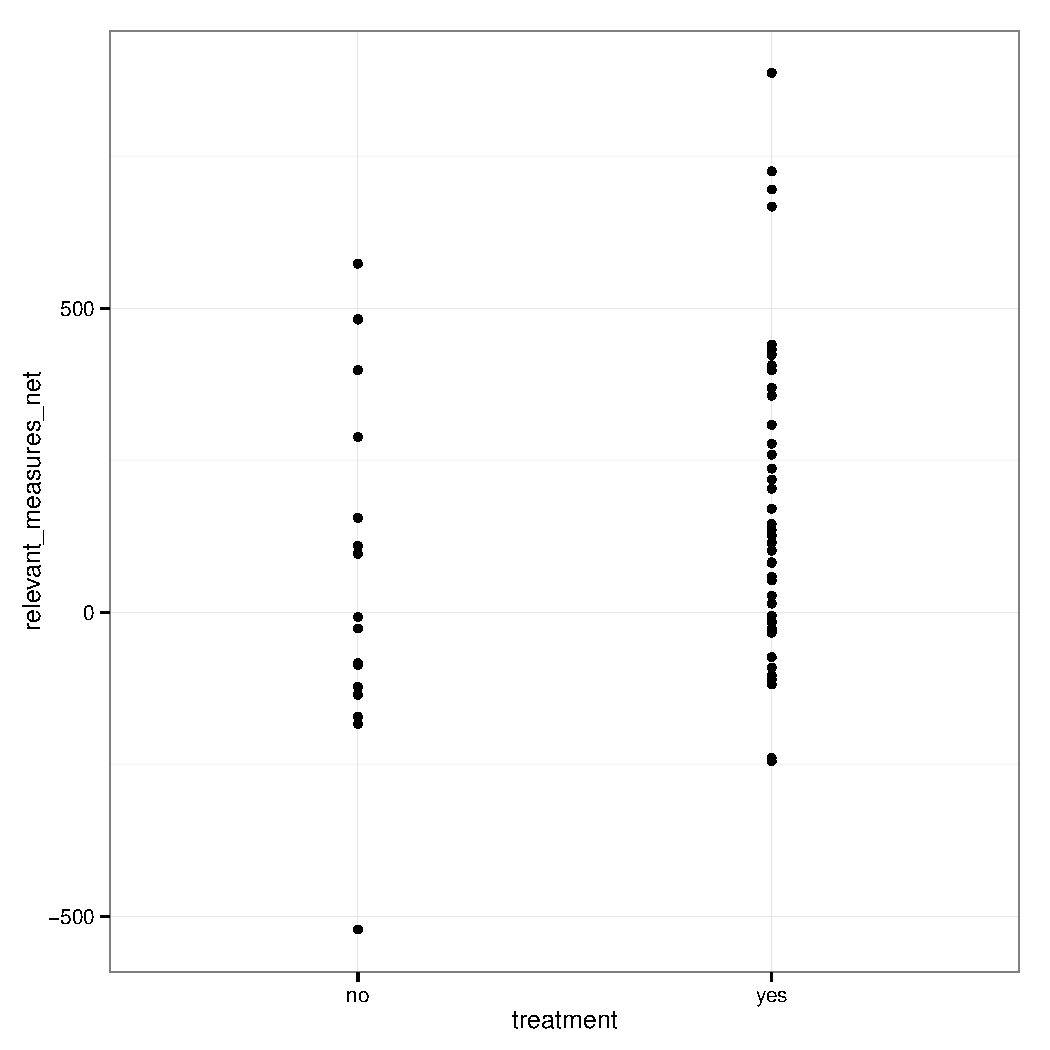
\includegraphics[width=4in,height=4in]{figure/PS13-unnamed-chunk-2-1} 

}



\end{knitrout}


\item Interpret the graph in part (a).\\
Answer:\\
The mean of the treatment observations (164) is higher than the mean of the control observations (74), suggesting that the the treatment led to 90 more Democratic votes per precinct.  The amount of dispersion around the mean is similar in both groups.

\item Use randomization inference to test whether the apparent difference-in-means could
have occurred by chance under the sharp null hypothesis of no treatment effect for
any precinct. Interpret the results.
Answer:\\
\begin{knitrout}
\definecolor{shadecolor}{rgb}{0.969, 0.969, 0.969}\color{fgcolor}\begin{kframe}
\begin{alltt}
\hlkwd{library}\hlstd{(ri)}
\hlstd{middleton} \hlkwb{<-}
  \hlkwd{within}\hlstd{(middleton,\{}
    \hlstd{Z} \hlkwb{<-} \hlkwd{as.numeric}\hlstd{(treatment}\hlopt{==}\hlstr{"yes"}\hlstd{)}
    \hlstd{Y} \hlkwb{<-} \hlstd{relevant_measures_net}
  \hlstd{\})}

\hlcom{# Conduct Randomization Inference}
\hlkwd{set.seed}\hlstd{(}\hlnum{1234567}\hlstd{)}
\hlstd{perms} \hlkwb{<-} \hlkwd{with}\hlstd{(middleton,} \hlkwd{genperms}\hlstd{(}\hlkwc{Z} \hlstd{= Z))}
\end{alltt}
\begin{verbatim}
## Too many permutations to use exact method.
## Defaulting to approximate method.
## Increase maxiter to at least 1867897112363099 to perform exact estimation.
\end{verbatim}
\begin{alltt}
\hlstd{probs} \hlkwb{<-} \hlkwd{genprob}\hlstd{(perms)}
\hlstd{ate} \hlkwb{<-} \hlkwd{with}\hlstd{(middleton,} \hlkwd{estate}\hlstd{(}\hlkwc{Y}\hlstd{=Y,} \hlkwc{Z}\hlstd{=Z,} \hlkwc{prob} \hlstd{= probs))}
\hlstd{Ys} \hlkwb{<-} \hlkwd{with}\hlstd{(middleton,} \hlkwd{genouts}\hlstd{(}\hlkwc{Y} \hlstd{= Y,} \hlkwc{Z} \hlstd{= Z,} \hlkwc{ate} \hlstd{=} \hlnum{0}\hlstd{))}
\hlstd{distout} \hlkwb{<-} \hlkwd{gendist}\hlstd{(}\hlkwc{Ys}\hlstd{=Ys,} \hlkwc{perms}\hlstd{=perms,} \hlkwc{prob}\hlstd{=probs)}
\hlstd{result} \hlkwb{<-} \hlkwd{dispdist}\hlstd{(distout,} \hlkwc{ate}\hlstd{=ate)}
\hlstd{result}\hlopt{$}\hlstd{greater.p.value}
\end{alltt}
\begin{verbatim}
## [1] 0.1144
\end{verbatim}
\end{kframe}

{\centering 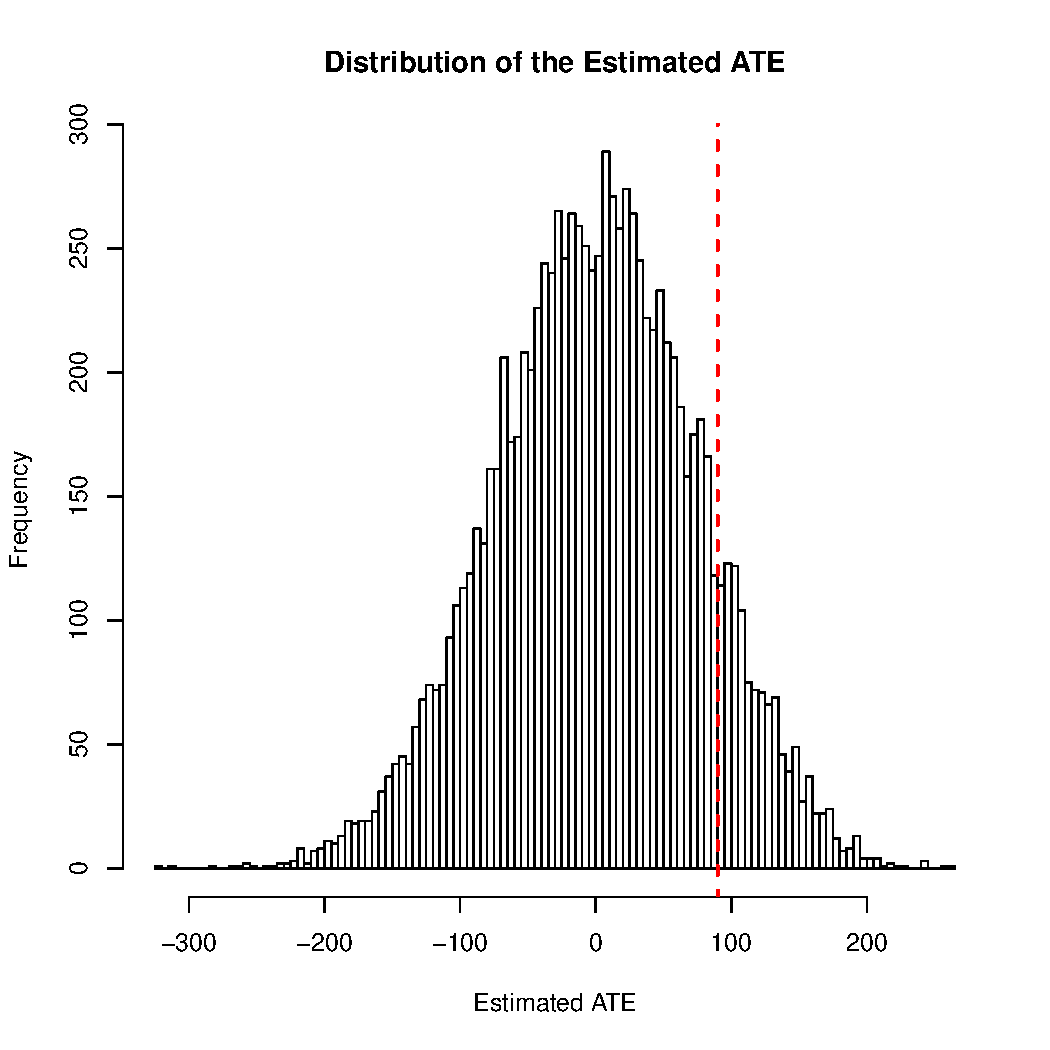
\includegraphics[width=4in,height=4in]{figure/PS13-unnamed-chunk-3-1} 

}



\end{knitrout}

A one-tailed test is appropriate here given that the campaign sought to increase its votes.  Randomization inference applied to 10,000 simulated randomizations shows that one-tailed p-value of the estimated ATE is 0.114. This figure is short of the conventional 0.05 threshold.

\item Suppose it were the case that when randomly assigning precincts, the authors used the following screening procedure: no random allocation was acceptable unless the average 2006 Democratic support score in the treatment group was within 0.5 percentage points of the average 2006 Democratic support score in the control group. Do all subjects have the same probability of being assigned to the treatment group? If not, re-estimate the ATE, weighting the data as described in Box 4.5. Redo your hypothesis test in part (c) subject to this restriction on the randomization. Interpret the results.\\
Answer:\\

\begin{knitrout}
\definecolor{shadecolor}{rgb}{0.969, 0.969, 0.969}\color{fgcolor}\begin{kframe}
\begin{alltt}
\hlcom{# Write restricted RA function}
\hlstd{restricted_ra} \hlkwb{<-} \hlkwa{function}\hlstd{()\{}
  \hlstd{middleton}\hlopt{$}\hlstd{Z_sim} \hlkwb{<-} \hlkwd{ifelse}\hlstd{(}\hlnum{1}\hlopt{:}\hlnum{65} \hlopt \hlkwd{sample}\hlstd{(}\hlnum{1}\hlopt{:}\hlnum{65}\hlstd{,} \hlnum{48}\hlstd{),} \hlnum{1}\hlstd{,} \hlnum{0}\hlstd{)}
  \hlcom{# check condition}
  \hlstd{fit} \hlkwb{<-} \hlkwd{lm}\hlstd{(dem_perf_06} \hlopt{~} \hlstd{Z_sim,} \hlkwc{data}\hlstd{=middleton)}
  \hlkwa{if}\hlstd{(}\hlkwd{abs}\hlstd{(}\hlkwd{coef}\hlstd{(fit)[}\hlnum{2}\hlstd{])} \hlopt{<} \hlnum{0.5}\hlstd{)\{}\hlkwd{return}\hlstd{(middleton}\hlopt{$}\hlstd{Z_sim)\}}
  \hlcom{# if condition is not met, call restricted_ra again}
  \hlkwd{return}\hlstd{(}\hlkwd{restricted_ra}\hlstd{())}
\hlstd{\}}

\hlkwd{set.seed}\hlstd{(}\hlnum{1234567}\hlstd{)}
\hlstd{perms} \hlkwb{<-} \hlkwd{genperms.custom}\hlstd{(}\hlkwc{randfun} \hlstd{= restricted_ra)}
\hlstd{probs} \hlkwb{<-} \hlkwd{genprob}\hlstd{(perms)}
\hlcom{# Restricted randomization changes the probabilities that each unit enters into treatment.}
\hlcom{# Here is the distribution of probabilities:}
\hlkwd{summary}\hlstd{(probs)}
\end{alltt}
\begin{verbatim}
##    Min. 1st Qu.  Median    Mean 3rd Qu.    Max. 
##  0.7281  0.7346  0.7370  0.7385  0.7430  0.7641
\end{verbatim}
\begin{alltt}
\hlstd{ate} \hlkwb{<-} \hlkwd{with}\hlstd{(middleton,} \hlkwd{estate}\hlstd{(}\hlkwc{Y}\hlstd{=Y,} \hlkwc{Z}\hlstd{=Z,} \hlkwc{prob} \hlstd{= probs))}
\hlstd{Ys} \hlkwb{<-} \hlkwd{with}\hlstd{(middleton,} \hlkwd{genouts}\hlstd{(}\hlkwc{Y} \hlstd{= Y,} \hlkwc{Z} \hlstd{= Z,} \hlkwc{ate} \hlstd{=} \hlnum{0}\hlstd{))}
\hlstd{distout} \hlkwb{<-} \hlkwd{gendist}\hlstd{(}\hlkwc{Ys}\hlstd{=Ys,} \hlkwc{perms}\hlstd{=perms,} \hlkwc{prob}\hlstd{=probs)}
\hlstd{result} \hlkwb{<-} \hlkwd{dispdist}\hlstd{(distout,} \hlkwc{ate}\hlstd{=ate)}
\hlstd{result}\hlopt{$}\hlstd{greater.p.value}
\end{alltt}
\begin{verbatim}
## [1] 0.022
\end{verbatim}
\end{kframe}

{\centering 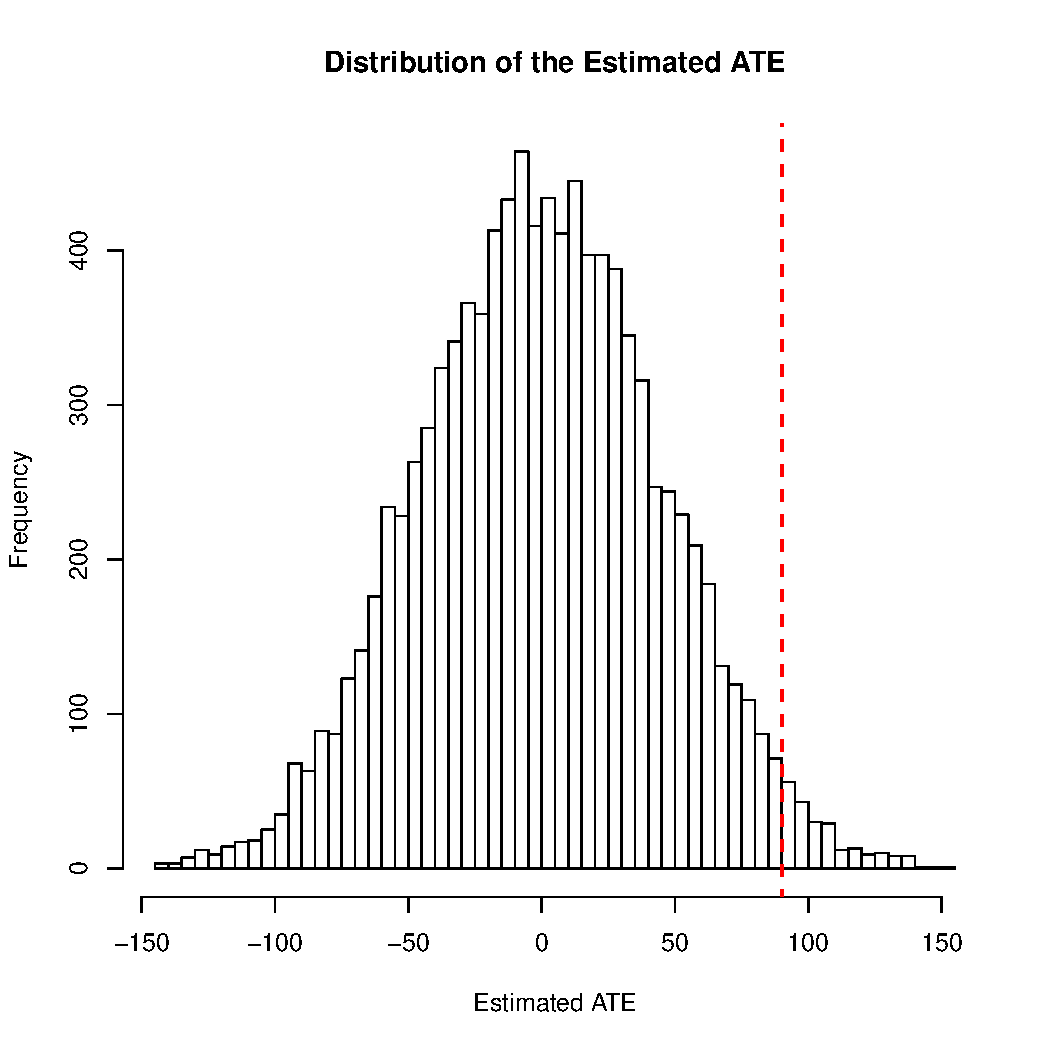
\includegraphics[width=4in,height=4in]{figure/PS13-unnamed-chunk-4-1} 

}



\end{knitrout}

Randomization inference applied to 10,000 simulated restricted randomizations shows that one-tailed p-value of the estimated ATE is 0.022. This figure allows us to reject the null hypothesis at the conventional 0.05 threshold.  The p-value here is lower than when we assume unrestricted randomization because re-randomization functions as a form of blocking..
\end{enumerate}

\section*{Question 2}
Select a published article that presents the design and analysis of a field experiment. Based on the publication and any supplementary materials provided by the authors, try to fill in as much of the reporting checklist for research articles as you can. What pieces of information, if any, went unreported? Does the failure to address one or more items on the checklist affect the confidence that you place in the results they report?\\
Answer:\\
Answers to this question will vary.


\section*{Question 3}
Conduct your own randomized experiment, based on one of the suggested topics in Appendix B.
\begin{enumerate}[a)]
\item Compose a planning document.
\item Take an online research ethics course, and obtain your certification to conduct human subjects research. Obtain approval for your study from the institutional review board at your college or university.
\item Conduct a small pilot study to work out any problems in administering the treatment or measuring outcomes.
\item Conduct the experiment. Construct a data file and supporting metadata.
\item Compose a research report.
\end{enumerate}
Answer:\\
Answers to this question will vary.



\end{document}

